
\chapter{Boxen, tabellen en figuren}

\section{Boxen}\index{box}\label{boxen}

Een box is een stuk tekst dat door \latex als ��n enkel karakter behandeld wordt. Boxen worden gebruikt om speciale opmaakeffecten te bekomen. De meeste schrijvers hoeven geen boxen te gebruiken (met uitzondering van een \lcommand{\\mbox} om dingen bij elkaar te houden). Het is pas wanneer je rare dingen wilt doen, dat boxen van pas kunnen komen.

\subsection{Links-rechts boxen}

Links-rechts boxen bevatten de tekst van links naar rechts (zij printen dus al hun tekst af op ��n enkele lijn). De syntax is:\index{mbox@\lcommand{\\mbox}}\index{fbox@\lcommand{\\fbox}}\index{makebox@\lcommand{\\makebox}}\index{framebox@\lcommand{\\framebox}}
\begin{llt}
\mbox{tekst}
\fbox{tekst}
\makebox[breedte][tekstpositie]{tekst}
\framebox[breedte][tekstpositie]{tekst}
\end{llt}
Met \lcommand{\\mbox} wordt de tekst in een box gezet. Om een kadertje te krijgen rond een box, kan \fbox{\lcommand{\\fbox}} gebruikt worden. Met \lcommand{\\makebox} (analoog aan \lcommand{\\mbox}) en \lcommand{\\framebox} (analoog aan \lcommand{fbox}), kan de breedte van de box meegegeven worden. De tekstpositie geeft aan hoe de tekst in de box uitgelijnd wordt: \lcommand{c} voor gecentreerd (standaard), \lcommand{l} voor links uitgelijnd, \lcommand{r} voor rechts uitgelijnd en \lcommand{s} om de tekst uit te vullen. Een voorbeeld:
\begin{llt}
------\framebox[2mm][c]{centrum}------
\end{llt}
geeft ------\framebox[2mm][c]{centrum}------. We zien dat \latex ervan uitgaat dat de box slechts 2mm breed is, ook al is de tekst eigenlijk breder (om dit te illustreren, werden rondom de box gedachtenstreepjes aangebracht).
\npar
Boxen kunnen ook naar boven verplaatst worden:\index{raisebox@\lcommand{\\raisebox}}
\begin{llt}
\raisebox{1ex}{Duc in altum!}
\raisebox{-1ex}{Errare humanum est, perseverare in errore diabolicum.}
\end{llt}
Het eerste argument bevat de hoogte waarmee de box moet verplaatst worden (in \latex-eenheden, zie bladzijde \pageref{latex-eenheden}), het tweede bevat de tekst. Het resultaat van het eerste voorbeeld is: \raisebox{1ex}{Duc in altum!}. Het tweede voorbeeld toont aan dat er ook gewerkt kan worden met negatieve hoogten: \raisebox{-1ex}{Errare humanum est, perseverare in errore diabolicum.}

\subsection{Parboxen en minipagina's}\label{parbox}

Om hele paragrafen in een box te zetten, kan gebruik gemaakt worden van het \lcommand{\\parbox}\index{parbox@\lcommand{\\parbox}} commando en de \lcommandx{minipage} omgeving. Parboxen worden gebruikt voor kortere stukken tekst, minipages voor langere stukken. Maar eigenlijk doen ze allebei hetzelfde. Hun syntax is als volgt:
\begin{llt}
\parbox[positie][hoogte][verticale-tekstpositie]{breedte}{tekst}

\begin{minipage}[positie][hoogte][verticale-tekstpositie]{breedte}
tekst
\end{minipage}
\end{llt}
Argumenten tussen vierkante haakjes zijn niet verplicht. De betekenis van de argumenten is de volgende:
\begin{description}
\item[positie] De positie van de box ten opzichte van de omliggende tekst. Met \lcommand{b} hangt de box uit de tekstlijn, met \lcommand{t} ligt ze erop en met \lcommand{c} zit ze er tussenin. Dit laatste is de standaard. Meer uitleg over de \emph{positie} parameter is de vinden in de sectie over tabellen (sectie \ref{positie}).
\item[hoogte] Hier kan de hoogte van de box ingegeven worden (in \latex eenheden, zie bladzijde \pageref{latex-eenheden}).
\item[verticale-tekstpositie] Deze parameter kan alleen worden meegegeven wanneer ook de vorige werd gegeven en bepaalt hoe de tekst in de box wordt geplaatst (ervan uitgaande dat de box te groot is). Er zijn vier mogelijkheden:
\begin{description}
\item[t] De tekst wordt tegen de top van de box geduwd: \fbox{\parbox[c][4ex][t]{15ex}{Plafondplakker}}, gemaakt met \lcommand{\\parbox\[c\]\[4ex\]\[t\]\{15ex\}\{Plafondplakker\}}
\item[b] De tekst wordt tegen de vloer van de box geduwd: \fbox{\parbox[c][4ex][b]{12ex}{Landpladijs}}, gemaakt met \lcommand{\\parbox\[c\]\[4ex\]\[b\]\{12ex\}\{Landpladijs\}}
\item[c] De tekst wordt verticaal gecentreerd in de box: \fbox{\parbox[c][4ex][c]{16ex}{In medio virtus}}, gemaakt met \lcommand{\\parbox\[c\]\[4ex\]\[c\]\{16ex\}\{In medio virtus\}}
\item[s] De tekst wordt uitgerekt zodat de hele box wordt bestreken. Er moet minimum ��n rubberen lengte voorkomen (zie sectie \ref{latex-eenheden} op bladzijde \pageref{latex-eenheden}) zodat de tekst daar kan uitgerekt worden.
\end{description}
\item[breedte] Hierin moet (verplicht argument) de breedte van de box worden ingegeven.
\end{description}

\subsection{Nesten van boxen}

De verschillende boxen kunnen in elkaar genest worden. Om bijvoorbeeld een kadertje te krijgen rondom een \lcommand{\\parbox}, zet je die in een \lcommand{fbox}:

\begin{center}
\fbox{\parbox{30em}{\lcommand{\\fbox\{\\parbox\{30em\}\{...\}\}}
\npar
Het commando hierboven is wat gebruikt werd voor het genereren van deze box, met uitzondering van de drie puntjes. Maar indien we de drie puntjes willen vervangen door de letterlijke tekst die in deze box voorkomt, krijgen we deze cursus nooit af.
}}
\end{center}
Om een box te maken die dezelfde breedte heeft als de lopende tekst, kan het commando \lcommand{\\textwidth} handig zijn.\index{textwidth@\lcommand{\\textwidth}} Dat bevat namelijk de breedte van de tekst:
\npar
\fbox{\parbox{\textwidth}{\lcommand{\\fbox\{\\parbox\{\\textwidth\}\{...\}\}}}}
\npar
Deze breedte kan ook vermenigvuldigd worden met een getal:
\npar
\fbox{\parbox{0.8\textwidth}{\lcommand{\\fbox\{\\parbox\{0.8\\textwidth\}\{...\}\}}}}

\section{Tabellen}\label{tabellen}

\subsection{Opbouwen van tabellen}\label{tabular}

De omgevingen \lcommandx{tabular}, \lcommand{tabular*} en \lcommandx{array} vormen de basis van waaruit elke tabel wordt opgebouwd. Hun syntax is als volgt:
\begin{llt}
\begin{array}[positie]{kols}                rijen       \end{array}
\begin{tabular}[positie]{kols}              rijen       \end{tabular}
\begin{tabular*}{breedte}[positie]{kols}    rijen       \end{tabular*}
\end{llt}
De \lcommand{array} omgeving kan enkel toegepast worden in \engels{math mode} (zie hoofdstuk \ref{math-mode}), maar wordt hier vermeld omdat de syntax dezelfde is als voor de \lcommand{tabular} omgeving. De betekenis van de verschillende gebruikte argumenten is:

\begin{description}\label{positie}
\item[positie] Elke tabel wordt door \latex beschouwd als ��n grote letter. Het is een nogal grote `letter', vandaar dat die een bepaalde positie moet krijgen op de lijn: \textbf{t}op, \textbf{b}ottom of \textbf{c}entreren.
\begin{description}
\item[t] De top van de tabel is gealigneerd met de basistekstlijn. Dit betekent dat de tabel uit de tekstlijn `hangt' \begin{tabular}[t]{|c|} \hline galg \\ \hline  galg \\ \hline \end{tabular}, zoals dit voorbeeld.
\item[b] De onderkant van de tabel is gealigneerd met de basistekstlijn. De tabel schiet naar boven, \begin{tabular}[b]{|c|} \hline pisa \\ \hline pisa \\ \hline \end{tabular}, zoals dit voorbeeld.
\item[c] Het midden van de tabel is gealigneerd met de basistekstlijn, zoals te zien is in dit voorbeeld: \begin{tabular}[c]{|c|} \hline pisa \\ \hline  galg \\ \hline \end{tabular}
\end{description}
Het positie-argument is optioneel (te zien aan de vierkante haakjes). Wanneer het niet wordt meegegeven, wordt standaard het midden van de tabel gealigneerd met de basistekstlijn (de \lcommand{c} optie).
\begin{MinderBelangrijk}
\item[breedte] Dit speelt alleen maar mee in de \lcommand{tabular*} omgeving. Het bepaalt de totale breedte van de tabel. In dit geval moet het \lcommand{kols} argument minstens ��n \lcommand{@\{extracolsep\{\\fill\}\}} bevatten. Bij de twee andere tabellen wordt de breedte bepaald door de inhoud.
\end{MinderBelangrijk}
\item[kols] Voor elke kolom moet worden aangegeven of de tekst rechts of links uitgelijnd wordt, of gecentreerd wordt. Verder kan het ook nodig zijn om de randen van de tabel te versieren, of om extra spati�ring (of speciale tekens) te voorzien tussen de kolommen. Dit wordt allemaal meegegeven in het \lcommand{kols} argument. De positie van de tekst in de kolommen kan bepaald worden met de volgende formatteringssymbolen:
\begin{description}
\item[l] De tekst wordt links uitgelijnd.
\item[r] De tekst wordt rechts uitgelijnd.
\item[c] De tekst wordt gecentreerd.
\item[p\{breed\}] De tekst wordt uitgevuld over een breedte `breed', die uitgedrukt wordt in de typische \latex lengte eenheden (zie bladzijde \pageref{latex-eenheden}).
\item[*\{aantal\}\{kols\}] Luiheid is de moeder van de vooruitgang. Als je de formattering van 10 dezelfde kolommen moet opnieuw schrijven, is dat nogal lastig. Gemakkelijker is als je die ��n keer ingeeft en dan zegt hoeveel keer je die kolom wilt hebben. Bijvoorbeeld \lcommand{rlrlrlrlrl} kan korter geschreven worden als \lcommand{*\{5\}\{rl\}}
\end{description}
Soms is het gewenst dat in elke rij een bepaald symbool terugkomt (zoals een verticale lijn, of een punt van de kommagetallen). Hiervoor kan het volgende in het \lcommand{kols} argument gestoken worden.
\begin{description}
\item[$\mid$] Zet een verticale lijn op die plaats.
\item[$\mid\;\mid$] Zet een dubbele verticale lijn op die plaats. Merk op dat verticale lijnen typografisch nooit zeer mooi zijn in een tabel, en dat ze meestal niet nodig zijn voor de leesbaarheid. Zo weinig mogelijk gebruiken dus.
\item[@\{text\}] Zet op die plaats in elke rij de tekst `text'. Dit is een zogenaamde @-uitdrukking. \latex zet tussen elke kolom witte ruimte (zodat de tekst van de verschillende kolommen niet aaneen plakt). Met een @-uitdrukking valt deze witte ruimte weg. Als we die willen bewaren, moeten we in de @-uitdrukking een witte ruimte opnemen (met \lcommand{\\hspace\{lengte\}}).\index{extracolsep} Langs de andere kant, als deze witte ruimte niet wenselijk is tussen bepaalde kolommen, kan ze worden teniet gedaan met \lcommand{@\{\}}.
\begin{MinderBelangrijk}
\npar
Met \lcommand{@\{\\extracolsep\{breed\}\}} wordt er in elke kolom die volgt op deze uitdrukking, een witte ruimte van breedte \lcommand{breed} ingevoegd totdat een andere \lcommand{@\{\\extracolsep\{breed\}\}} ingegeven wordt. Deze extra spati�ring wordt niet verwijderd wanneer andere @-uitdrukkingen gebruikt worden. In een \lcommand{tabular*} omgeving moet er ergens een \lcommand{@\{\\extracolsep\{\\fill\}\}} voorkomen, zodat de breedte van de daaropvolgende kolommen kan uitgerekt worden opdat de tabel de voorgedefinieerde breedte kan aannemen.
\end{MinderBelangrijk}
\end{description}
\item[rijen] Hier worden de verschillende rijen van de tabel ingegeven. Elke rij wordt afgesloten met \lcommand{\\\\} (twee rechten met een negatieve richtingsco�ffici�nt) of met het commando \lcommand{\\tabularnewline}.\index{tabularnewline@\lcommand{\\tabularnewline}} De verschillende kolommen in een rij worden gesplitst door \lcommand{&} tekens. Elke rij bevat juist evenveel kolommen als het aantal gedefinieerd bij het begin van de tabel. Sommige elementen mogen leeg zijn (aangegeven door twee opeenvolgende \& tekens). In de rijen kunnen bepaalde speciale commando's gegeven worden om horizontale lijnen te trekken en om cellen samen te nemen.\index{\&}\index{\\@\lcommand{\\\\}} 
\begin{itemize}
\item[]\hspace{-\labelwidth}\hspace{-\labelsep}\lcommand{\\hline}\hspace{\labelsep} Dit commando mag alleen geplaatst worden in het begin van een rij. Het zorgt voor een horizontale lijn over de volledige breedte van de tabel. Twee \lcommand{\\hline} commando's na elkaar zorgen voor een dubbele horizontale lijn. \index{hline@\lcommand{\\hline}}
\item[]\hspace{-\labelwidth}\hspace{-\labelsep}\lcommand{\\cline\{m-n\}}\hspace{\labelsep} Dit commando plaatst een horizontale lijn vanaf het begin van kolom \lcommand{m} tot het einde van kolom \lcommand{n}. Het mag alleen gebruikt worden in het begin van een rij. Het mag meerdere keren gebruikt worden op dezelfde rij.
\item[]\hspace{-\labelwidth}\hspace{-\labelsep}\lcommand{\\vline}\hspace{\labelsep} Dit commando plaatst een verticale lijn met dezelfde hoogte als de rij. Op die manier kunnen verticale lijnen verkregen worden die niet doorlopen over heel de hoogte van de tabel.
\item[]\hspace{-\labelwidth}\hspace{-\labelsep}\lcommand{\\multicolumn\{aantal\}\{kols\}\{text\}}\hspace{\labelsep} Dit commando combineert het `aantal' kolommen volgend op de plaats waar het gegeven wordt, in ��n kolom. Deze kolom moet juist ��n specificatie krijgen zoals gedefinieerd in \lcommand{kols}. Het kan ook gebruikt worden om in juist ��n cel, de tekstuitlijning te wijzigen. Hiertoe wordt `aantal' gelijk aan 1 gekozen.\index{multicolumn@\lcommand{\\multicolumn}} 
\end{itemize}
\end{description}

\begin{MinderBelangrijk}

\subsection{Stijlparameters voor tabellen}

De stijlparameters die \latex gebruikt voor het genereren van tabellen kunnen door de gebruiker gewijzigd worden. Deze parameters worden ofwel gewijzigd in de \engels{preamble}, zodat ze gelden voor het hele document, ofwel lokaal rond de \lcommand{tabular} omgeving (in een omgeving rondom). Echter nooit in de \lcommand{tabular} omgeving zelf. Bijvoorbeeld zo:
\begin{llt}
{                               % Begin omsluitende omgeving
\setlength{\tabcolsep}{5pt}     % Spatie tussen kolommen
\begin{tabular}{ccc}            % Begin tabular omgeving
    een & twee & drie           % De rijen
\end{tabular}                   % Einde tabular omgeving
}                               % Einde omsluitende omgeving
\end{llt}
De verschillende lengteparameters die kunnen gewijzigd worden, zijn:
\begin{itemize}
\item \lcommand{\\tabcolsep}\index{tabcolsep@\lcommand{\\tabcolsep}}\hspace{\labelsep} De helft van de ruimte die tussen de verschillende kolommen wordt aangebracht. Geldt enkel voor de \lcommand{tabular} en \lcommand{tabular*} omgeving.
\item \lcommand{\\arraycolsep}\index{arraycolsep@\lcommand{\\arraycolsep}}\hspace{\labelsep} Analoog als \lcommand{\\tabcolsep} maar dan voor de \lcommand{array} omgeving.
\item \lcommand{\\arrayrulewidth}\index{arrayrulewidth@\lcommand{\\arrayrulewidth}}\hspace{\labelsep} De dikte van de horizontale en verticale lijnen in een tabel.
\item \lcommand{\\doublerulesep}\index{doublerulesep@\lcommand{\\doublerulesep}}\hspace{\labelsep} De witte ruimte tussen twee opeenvolgende lijnen.
\end{itemize}
Het wijzigen van de afstand tussen de verschillende rijen, gebeurt met
\begin{llt}
\renewcommand{\arraystretch}{factor}
\end{llt}
Hierbij is \lcommand{factor} standaard gelijk aan 1.\index{arraystretch@\lcommand{\\arraystretch}} Dezelfde uitleg als voor \lcommand{\\baselinestretch} (bladzijde \pageref{baselinestretch}) geldt hier.
\end{MinderBelangrijk}

\subsection{Voorbeelden} \label{voorbeelden-tabellen}

Tabellen produceren lijkt moeilijk, maar is zeer gemakkelijk. Eigenlijk schrijf je gewoon hoe de tabel er moet uit zien. We zullen nu enkele voorbeelden geven. Links geven we de tabel, rechts de \latex code nodig om de tabel te genereren.

\subsubsection{Decimale getallen, het gebruik van de @-uitdrukking}

Het wetenschappelijk ordenen van decimale getallen in een kolom, eist dat de decimale tekens onder elkaar vallen. Dit kan als volgt verkregen worden:

\begin{minipage}{0.4\textwidth} \begin{center}
\begin{tabular}{r@{.}l}
987     & 75025\\
514229  & 13
\end{tabular}
\end{center}\end{minipage}
\quad
\begin{minipage}{0.58\textwidth}\begin{llt}
\begin{tabular}{r@{.}l}
987     & 75025\\
514229  & 13
\end{tabular}
\end{llt}\end{minipage}

De eerste kolom wordt rechts uitgelijnd, dan wordt een punt geplaatst (de @-expressie zorgt daarvoor) en tenslotte worden de cijfers van de derde kolom links tegen het punt geduwd.
\npar
Een @-uitdrukking kan ook gebruikt worden om telkens hetzelfde te laten verschijnen in een kolom:

\begin{minipage}{0.4\textwidth} \begin{center}
\begin{tabular}{l@{ = }r}
F10     & 55\\
F11     & 89
\end{tabular}
\end{center}\end{minipage}
\quad
\begin{minipage}{0.58\textwidth}\begin{llt}
\begin{tabular}{l@{ = }r}
F10     & 55\\
F11     & 89
\end{tabular}
\end{llt}\end{minipage}

Merk echter op dat een kolom waarin veel keer hetzelfde voorkomt, kan vervangen worden door extra uitleg in het bijschrift van de tabel.

\subsubsection{Samenvoegen van cellen}

Voor bijvoorbeeld multidimensionale tabellen kan het samenvoegen van cellen handig zijn:

\begin{minipage}{0.4\textwidth} \begin{center}
\begin{tabular}{lrrr}
      & \multicolumn{3}{c}{Metingen}  \\
F10   & 55    & 54    & 56            \\
F11   & 89    & 90    & 88
\end{tabular}
\end{center}\end{minipage}
\quad
\begin{minipage}{0.58\textwidth}\begin{llt}
\begin{tabular}{lrrr}
      & \multicolumn{3}{c}{Metingen}  \\
F10   & 55    & 54    & 56            \\
F11   & 89    & 90    & 88
\end{tabular}
\end{llt}\end{minipage}

De eerste cel van de eerste rij is leeg. De drie volgende cellen worden samen genomen en vervangen door ��n cel waarbinnen de tekst gecentreerd staat (die \lcommand{\{c\}}). Met kommagetallen kan dit ook, dit bewijst het volgende voorbeeld waarin ook het gebruik van \lcommand{*\{aantal\}\{kols\}} wordt getoond:

\begin{minipage}{0.4\textwidth} \begin{center}
\begin{tabular}{l*{3}{r@{.}l}}
      & \multicolumn{6}{c}{Metingen}       \\
F10   & 55  & 3   & 54   & 5   & 56   & 8  \\
F11   & 89  & 13  & 90   & 21  & 88   & 34
\end{tabular}
\end{center}\end{minipage}
\quad
\begin{minipage}{0.58\textwidth}\begin{llt}
\begin{tabular}{l*{3}{r@{.}l}}
      & \multicolumn{6}{c}{Metingen}       \\
F10   & 55  & 3   & 54   & 5   & 56   & 8  \\
F11   & 89  & 13  & 90   & 21  & 88   & 34
\end{tabular}
\end{llt}\end{minipage}

We beginnen met een links uitgelijnde kolom. We doen verder met \lcommand{*\{3\}\{r@\{.\}l\}}. Dit zijn in totaal 6 kolommen. Drie keer een rechtsuitgelijnde kolom, gevolgd door een punt, gevolgd door een linksuitgelijnde kolom. Daarom dat we bij \lcommand{\\multicolumn} aangeven dat we 6 kolommen wensen samen te voegen (het punt telt niet mee bij de kolomtelling).
\npar
Het samenvoegen van cellen in verticale richting is niet direct mogelijk. Er bestaan natuurlijk wel omwegen: het is perfect toegelaten om een tabel binnen een andere tabel te gebruiken (geneste tabellen):

\begin{minipage}{0.4\textwidth} \begin{center}
\begin{tabular}{l*{3}{r@{.}l}}
    \begin{tabular}{c} 
    Grootheid \\ (mm) \\
    \end{tabular}
      & \multicolumn{6}{c}{Metingen}       \\
F10   & 55  & 3   & 54   & 5   & 56   & 8  \\
F11   & 89  & 13  & 90   & 21  & 88   & 34
\end{tabular}
\end{center}\end{minipage}
\quad
\begin{minipage}{0.58\textwidth}\begin{llt}
\begin{tabular}{l*{3}{r@{.}l}}
    \begin{tabular}{c} 
    Grootheid \\ (mm) \\
    \end{tabular}
      & \multicolumn{6}{c}{Metingen}       \\
F10   & 55  & 3   & 54   & 5   & 56   & 8  \\
F11   & 89  & 13  & 90   & 21  & 88   & 34
\end{tabular}
\end{llt}\end{minipage}

Het eerste element is een tabelletje op zich. Terloops zien we ook dat elke rij niet op ��n tekstlijn moet staan. Voor grote tabellen is het zeer handig om de verschillende cellen op verschillende lijnen te plaatsen. Verder valt op dat in de minitabel, de verschillende kolommen in de input niet op verschillende lijnen staan. We kunnen de tabel zelfs op ��n lijn zetten in de broncode (dit wordt gedaan in het volgende voorbeeld). De opmaak in het bronbestand draagt niet bij tot de finale opmaak in het \bestand{pdf}-bestand.

\subsubsection{Lijntjes trekken}

In dit laatste voorbeeld tonen we hoe we gemakkelijk lijnen in onze tabel kunnen plaatsen:

\begin{minipage}{0.4\textwidth} \begin{center}
\begin{tabular}{l|*{3}{r@{.}l}}
\hline \hline % Horizontale dubbele lijn
  \begin{tabular}{c}
    Grootheid\\(mm)\\
  \end{tabular}
      & \multicolumn{6}{c}{Metingen}  \\
\hline % Horizontale lijn
F10   & 55  & 3 \vline & 
                54  & 5   & 56   & 8  \\
\cline{5-6} % Lijntje op kolom 5 en 6
F11   & 89  & 13       &\vline 
                90  & 21  & 88   & 34 \\
\hline \hline % Horizontale dubbele lijn
\end{tabular}
\end{center}\end{minipage}
\quad
\begin{minipage}{0.58\textwidth}\begin{llt}
\begin{tabular}{l|*{3}{r@{.}l}}
\hline \hline % Horizontale dubbele lijn
  \begin{tabular}{c}
    Grootheid\\(mm)\\ \end{tabular}
      & \multicolumn{6}{c}{Metingen}  \\
\hline % Horizontale lijn
F10   & 55  & 3 \vline & 
                54  & 5   & 56   & 8  \\
\cline{5-6} % Lijntje op kolom 5 en 6
F11   & 89  & 13       &\vline 
                90  & 21  & 88   & 34 \\
\hline \hline % Horizontale dubbele lijn
\end{tabular}
\end{llt}\end{minipage}

De tabel wordt omsloten door dubbele horizontale lijnen, geproduceerd door telkens twee keer na elkaar het commando \lcommand{\\hline} te geven. Na de hoofding volgt een enkele lijn (��n keer het commando \lcommand{\\hline}). Het valt op de merken dat er na een \lcommand{\\hline} commando geen \lcommand{\\\\} moet volgen. Met \lcommand{\\cline\{5-6\}} zorgen we voor een horizontale lijn in kolom 5 en 6. Dit commando moet gegeven worden in het begin van een rij en heeft invloed op de bovenkant van die rij. Door hier en daar \lcommand{\\vline} te gebruiken, kunnen we midden in de tabel van die verticale lijntjes trekken. Merk op dat die verticale lijnen nogal tegen de tekst plakken, veel meer dan wanneer een verticale lijn in de kolomspecificatie wordt gedefinieerd: \lcommand{l|} in \lcommand{\\begin\{tabular\}\{l|*\{3\}\{r@\{.\}l\}\}}.

\section{Figuren}\label{figuren}

Er bestaan \latex commando's om rechtstreeks figuren te tekenen:

\begin{minipage}{0.5\textwidth}
\begin{center}
\setlength{\unitlength}{1mm}
\begin{picture}(40,40)
\put(0,0){\line(1,0){40}}
\put(0,0){\line(1,2){20}}
\put(0,0){\line(3,2){30}}
\put(20,0){\line(0,1){40}}
\put(40,0){\line(-1,2){20}}
\put(40,0){\line(-3,2){30}}
\put(20,13.5){\circle{5}}
\put(20,13.5){\circle*{2}}
\end{picture}
\end{center}
\end{minipage}
\begin{minipage}{0.5\textwidth}
\begin{llt}
\setlength{\unitlength}{1mm}
\begin{picture}(40,40)
\put(0,0){\line(1,0){40}}
\put(0,0){\line(1,2){20}}
\put(0,0){\line(3,2){30}}
\put(20,0){\line(0,1){40}}
\put(40,0){\line(-1,2){20}}
\put(40,0){\line(-3,2){30}}
\put(20,13.5){\circle{5}}
\put(20,13.5){\circle*{2}}
\end{picture}
\end{llt}
\end{minipage}

Maar deze zijn niet handig in gebruik. Vandaar dat we ze hier ook niet gaan beschrijven. We zullen ons meer toespitsen op het importeren van figuren. Wanneer we met \command{pdflatex} werken, en dus rechtstreeks pdf's produceren (zie bladzijde \pageref{compileren}), kunnen we verschillende soorten figuren importeren: \begrip{pdf} (ja, figuren kunnen ook bewaard worden in pdf's, dit is trouwens het te verkiezen formaat, daar het vectorgericht is), \begrip{png} (beste formaat voor pixelfiguren), \begrip{jpg}~\ldots  Wanneer we toch om ��n of andere reden met \command{latex} werken, kunnen we alleen \begrip{eps} bestanden invoegen.
\npar
Er bestaan twee pakketen voor het invoegen van figuren: \lcommandx{graphics} en \lcommand{graphicx}. Het eerste is iets verouderd. Daarom dat we hier alleen het tweede bespreken. Voor meer details verwijzen we naar het bestand \bestand{grfguide.ps},\footnote{Op een Debian systeem te vinden in: \bestand{/usr/share/doc/texmf/latex/graphics/grfguide.ps.gz}} te vinden in de meeste \latex distributies.
\npar
Om figuren te kunnen invoegen in het document, moet de volgende regel voorkomen in de \engels{preamble} (let op de \lcommand{x} op het einde van \lcommand{graphicx}):
\begin{llt}
\usepackage{graphicx}           % Om figuren te kunnen verwerken
\usepackage[draft]{graphicx}    % Draft mode
\end{llt}
Twee opties kunnen meegegeven worden: \begrip{draft} en \begrip{final}. In \engels{draft} mode wordt lege ruimte voorzien daar waar de figuren moeten komen, maar worden de figuren zelf niet ingevoegd. Wanneer je bezig bent met het goedzetten van tekst en de figuren voorlopig minder belangrijk zijn, kun je die optie aanzetten: dit versnelt het compileerproces danig. De optie \lcommand{final} zorgt ervoor dat alle figuren zeker in het pdf document verschijnen.
\npar
Het invoegen van een figuur in het document gebeurt met (hier een \lcommand{s} op het einde van \lcommand{\\includegraphics}):
\begin{llt}
\includegraphics{figuurnaam.png}
\end{llt}
\begin{MinderBelangrijk}
De extensie moet niet altijd meegegeven worden. \latex zoekt zelf naar \bestand{figuurnaam.pdf}. Als dat niet gevonden wordt zoekt de compiler naar \bestand{figuurnaam.png} en zo verder. In de \engels{preamble} kunnen we eventueel opgeven naar welke extensies moet gezocht worden:
\begin{llt}
\DeclareGraphicsExtensions{pdf, png, jpg, jpeg}
\end{llt}
Merk op dat het niet is omdat \latex de figuur vindt, dat ze ook verwerkt kan worden. Sommige figuren kunnen nu eenmaal niet ge�mporteerd worden. Zet ze met een ander programma om in bijvoorbeeld png of pdf formaat\footnote{Onder Unix is er het handige \command{convert} van de ImageMagick software. Voor het omzetten van eps naar pdf is echter \command{epstopdf} aangewezen~\ldots}.
\npar
\end{MinderBelangrijk}
Bij het invoegen van figuren zijn er een aantal opties die onontbeerlijk zijn:
\begin{description}
\item[width]\index{width} Is een \latex lengte (zie bladzijde \pageref{latex-eenheden} voor meer uitleg) en geeft aan hoe breed onze figuur moet zijn. Indien geen \lcommand{height} wordt opgegeven, behoudt de figuur zijn breedte--hoogte verhouding.
\item[height]\index{height} Is een \latex lengte en bepaalt hoe hoog onze figuur moet zijn. Indien geen breedte wordt opgegeven, behoudt de figuur zijn breedte--hoogte verhouding.
\item[angle]\index{angle} Is een getal dat aangeeft hoeveel graden de figuur moet gedraaid worden. De hoogte en de breedte draaien mee. Indien dus een hoogte of breedte wordt opgegeven en dan wordt een hoek van 90 graden gegeven, zal de hoogte de breedte worden en vice versa.
\item[totalheight] De totale hoogte van de figuur: wanneer een figuur gedraaid wordt, neemt de totale hoogte bijna altijd toe (vraag maar aan Pythagoras). Met \lcommand{height} wordt alleen de hoogte van de niet geroteerde figuur ingesteld terwijl met \lcommand{totalheight} de totale hoogte wordt ingesteld.
\end{description}
Al deze opties worden tussen vierkante haken ingegeven via de \engels{key=value} notatie:
\begin{llt}

\includegraphics[width=7cm]{cheops}
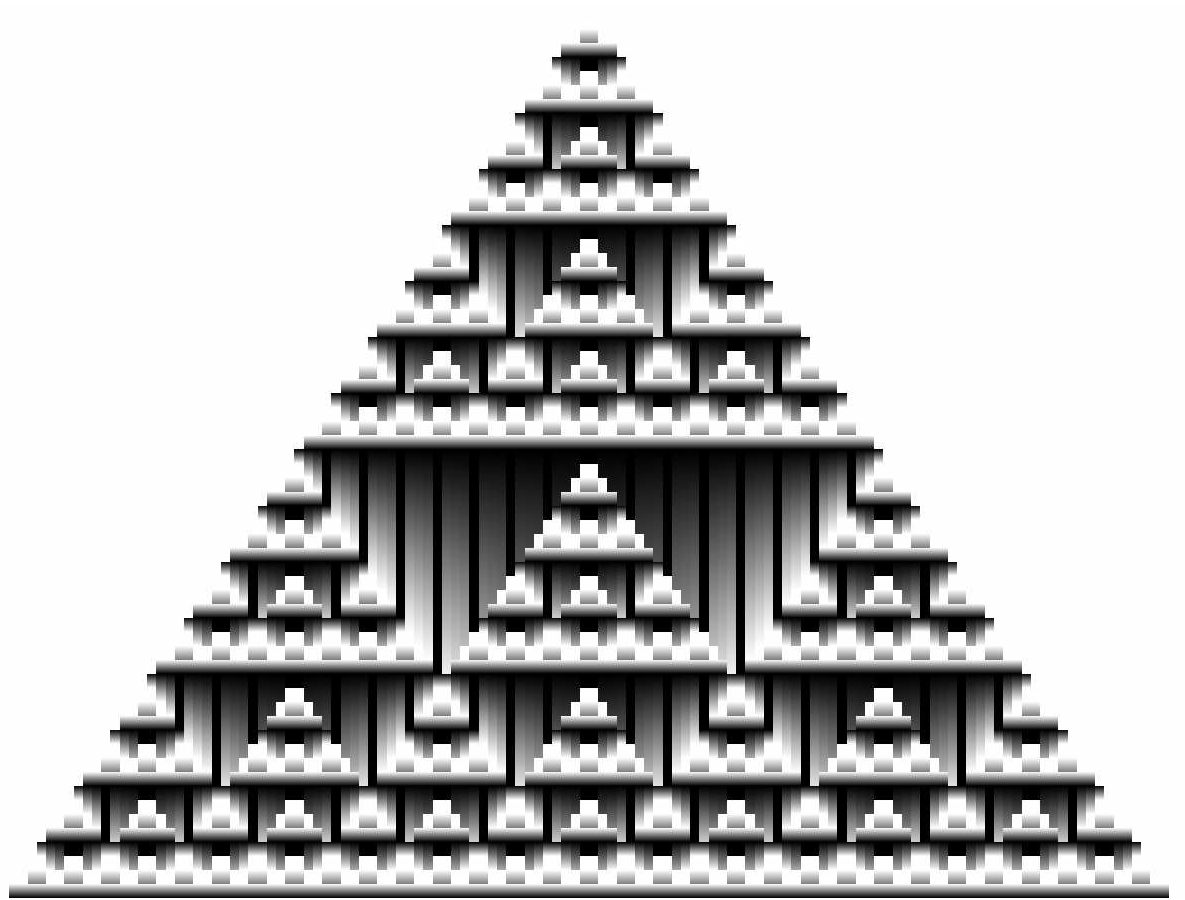
\includegraphics[width=0.5\textwidth]{chephren}
\end{llt}
\begin{figure}
\mbox{
\includegraphics[width=0.5\textwidth]{cheops}}
\mbox{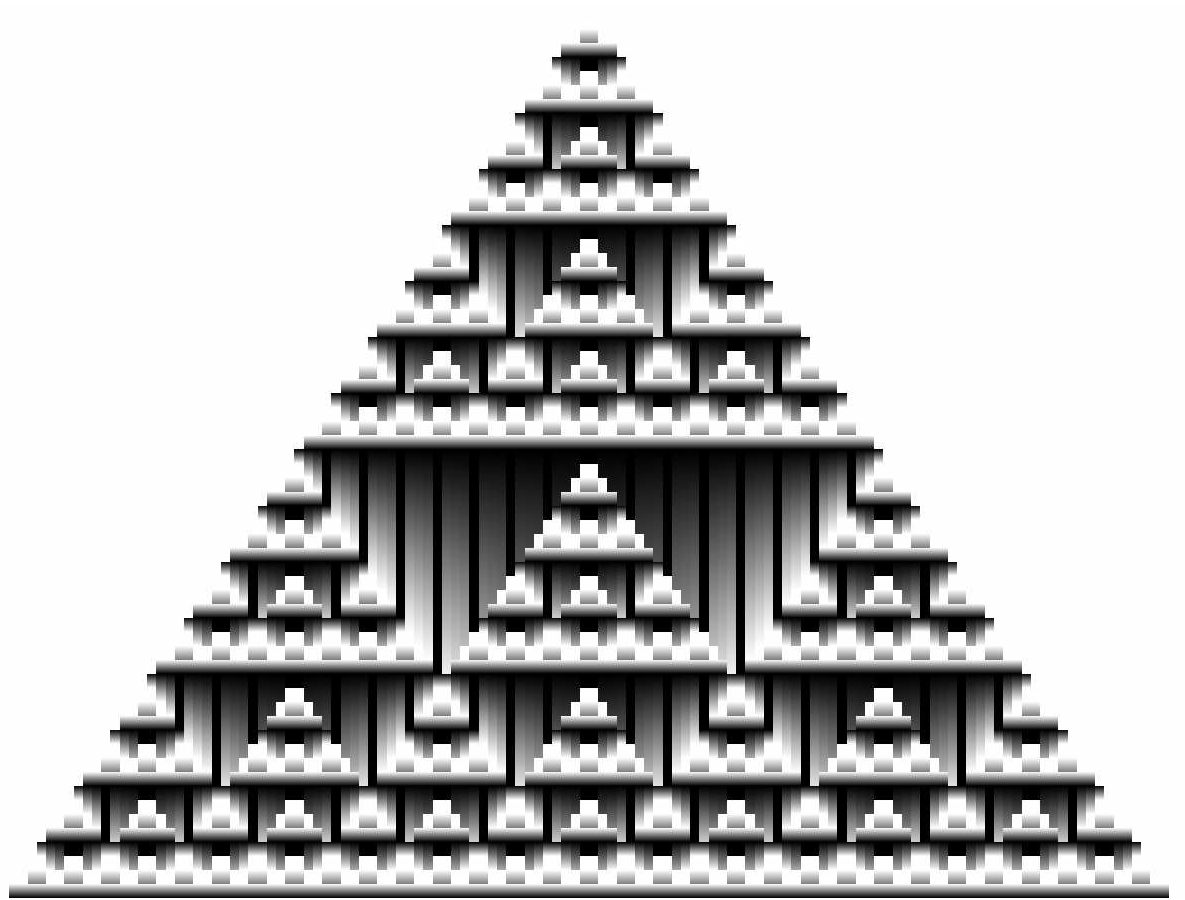
\includegraphics[width=0.5\textwidth]{chephren}}
\caption{Een figuur zegt {\scriptsize meestal} meer dan duizend woorden.}
\label{cheops-chephren}
\end{figure}
We zien dat we gebruik kunnen maken van de speciale lengte \lcommand{\\textwidth},\index{textwidth@\lcommand{\\textwidth}} die de breedte van de tekst weergeeft. De tweede figuur wordt even breed als de helft van de tekstbreedte. Het resultaat van deze commando's is te bezichtigen in figuur \ref{cheops-chephren}.
\npar
Figuren bewaren we best niet in de hoofdirectory van onze thesis. We maken bijvoorbeeld een subdirectory \bestand{figuren} aan. Zodus wordt het bovenstaande commando 
\begin{llt}
\includegraphics{figuren/figuurnaam}
\end{llt}
Niet zeer handig om altijd diezelfde directory te moeten intypen. Vandaar dat je in de \engels{preamble} kan opgeven in welke directories \latex naar figuren moet gaan zoeken:\label{graphicspath}
\begin{llt}
\graphicspath{{figuren/}{nog_een_dir_met_figuren/}}
\end{llt}
Wanneer de \latex compiler een figuur moet invoegen, gaat hij nu zoeken in de directory \bestand{figuren/} en in \bestand{nog_een_dir_met_figuren/}.
Merk op dat ook onder Windows de slash met een positieve richtingsco�ffici�nt moet gebruikt worden (en niet de \engels{backslash}).

\section{Zwevende tabellen en figuren}

\subsection{Zwevend maken}

Met de \lcommand{tabular} omgeving wordt de tabel daar geplaatst waar ze gedefinieerd werd. Met \lcommand{\\includegraphics} wordt de figuur daar geplaatst waar het commando gegeven werd. Als een tabel niet op de huidige bladzijde past, wordt een nieuwe bladzijde begonnen. Hetzelfde bij figuren. Dit kan zorgen voor nogal wat halflege bladzijden. Vandaar dat het beter is om de \latex compiler te laten beslissen waar de tabellen en figuren moeten geplaatst worden. Dit gebeurt via het zogenaamde \begrip{float} mechanisme. De tabellen en figuren worden in een \engels{float} omgeving geplaatst.
\npar
Voor tabellen wordt de \lcommandx{table} omgeving gebruikt:
\begin{llt}
\begin{table}[waar]
  \begin{tabular}{ccc}
   ... %  tabeltekst
  \end{tabular}
\end{table}
\end{llt}
Het genereren van de tabel zelf gebeurt zoals uitgelegd in sectie \ref{tabellen}.
Figuren worden in een \lcommandx{figure} omgeving geplaatst:
\begin{llt}
\begin{figure}[waar]
  \includegraphics[width=5cm]{vbfig01}
\end{figure}
\end{llt}
Op zich doen \lcommand{table} en \lcommand{figure} juist hetzelfde: ze nemen de tabel of figuur vast en zetten die op een typografisch verantwoorde plaats. Met het optionele argument (bemerk de vierkante haken) \lcommand{waar} kunnen we onze voorkeur uitdrukken over waar we de figuur graag zouden hebben. Het argument \lcommand{waar} kan uit verschillende letters bestaan. Deze letters zijn de volgende:\label{plaatsingfloat}
\begin{description}
\item[h] (Hier) De figuur of tabel mag op de plaats komen waar hij in de brontekst wordt ingegeven.
\item[t] (Top) De figuur of tabel mag aan de bovenkant van de huidige bladzijde komen, of als daar niet genoeg plaats is, aan het begin van de volgende bladzijde.
\item[b] (Beneden) De figuur of tabel mag aan de onderkant van de huidige bladzijde komen. Als daar niet genoeg plaats meer is, wordt de onderkant van de volgende bladzijde gebruikt.
\item[p] (Pagina) De figuur of tabel wordt opgespaard tot het einde van het hoofdstuk of sectie, waar een aantal bladzijden worden voorzien met alleen maar figuren en tabellen.
\item[!] Normaalgezien respecteert \latex een aantal regeltjes over de hoeveelheid \engels{floats} op een bladzijde, het aantal \engels{floats} in het begin van een pagina, en zo meer. Dit zorgt ervoor dat figuren en tabellen soms nogal ver van hun oorspronkelijke tekst geplaatst worden. Door een uitroepteken mee te geven met de positioneringsargumenten, zeggen we tegen \latex om geen rekening te houden met die typografische regels. We riskeren dan wel bladzijden te krijgen waar enkel \engels{floats} op staan.
\item[H] (Hier en nergens anders!) Soms willen we de tabel of figuur krijgen daar waar ze gedefinieerd wordt. Zelfs als daarvoor een nieuwe bladzijde moet begonnen worden. Deze optie is niet aanwezig in de standaard \latex maar moet opgeladen worden met een nieuw pakket met de originele naam \begrip{float}:
\begin{llt}
\usepackage{float}  % Om nieuwe float omgevingen aan te maken. Ook optie H!
\end{llt}
Dit pakket laat ook toe om eigen float omgevingen te maken, maar hiervoor verwijzen we naar de excellente documentatie van het pakket zelf.\footnote{Op een Debian systeem: \bestand{/usr/share/doc/texmf/latex/styles/float.dvi.gz}}
\end{description}
Dus met \lcommand{\\begin\{table\}\[ht!\] tabel \\end\{table\}} maken we een zwevende tabel die hier geplaatst wordt en als dat niet gaat, op de top van de volgende bladzijde. \latex moet zich ook niets aantrekken van typografische beperkingen in verband met \engels{floats}.

\subsection{Bijschrift}\index{bijschrift}\index{caption@\lcommand{\\caption}}

Het is altijd leuk als de lezers wat extra uitleg krijgen bij een tabel of figuur. Dit versieren gebeurt met het commando \lcommand{\\caption\{uitleg\}}. Bij de \lcommand{figure} omgeving genereert dit de titel \mbox{`Figuur 1.3: uitleg'} en bij de \lcommand{table} omgeving \mbox{`Tabel 1.3: uitleg'}. Traditioneel wordt een figuur versierd met een onderschrift en een tabel met een bovenschrift. Daarom dat bij een tabel het \lcommand{\\caption} commando wordt gegeven v��rdat de \lcommand{tabular} omgeving begint en bij een figuur n� de \lcommand{\\includegraphics}.
\npar
Standaard is het bijschrift in \latex niet echt te onderscheiden van de rest van het document (zelfde lettertype, zelfde lettergrootte, geen inspringing). Om hieraan te verhelpen, kan het pakket \lcommand{caption} gebruikt worden. Voor de uitgebreide mogelijkheden die dit pakket biedt, verwijzen we naar de uitstekende documentatie.\footnote{Op een Debian systeem: \url{/usr/share/doc/texmf/latex/caption/caption.pdf.gz}.}
\npar
Om \lcommand{caption} te gebruiken, is de volgende lijn nodig in de \engels{preamble}:
\begin{llt}
\usepackage[opties]{caption} 
\end{llt}
Hierbij zijn het \lcommand{opties} die de bijschriften van onze tabellen en figuren bepalen. De mogelijkheden zijn:
\begin{description}
\item[Stijl] De volgende argumenten kunnen gebruikt worden om te bepalen hoe het bijschrift wordt uitgelijnd.
\begin{description}
\item[normal] Volle regels worden uitgemiddeld. De laatste lijn wordt links uitgelijnd. Dit is zoals gewone tekst.
\item[flushleft] Alle regels worden tegen de linkerkantlijn geduwd.
\item[flushright]   Alle regels worden tegen de rechterkantlijn geduwd.
\item[center] Alle regels worden gecentreerd.
\item[centerlast] Alle regels worden uitgemiddeld. De laatste lijn wordt gecentreerd.
\item[hang] Hetzelfde als \lcommand{normal}, behalve dat vanaf de tweede regel van het bijschrift de tekst inspringt met een lengte gelijk aan die van de titel van het bijschrift.
\item[noonline] Al de bovenvermelde uitlijningsopties hebben alleen betrekking op bijschriften die meerdere regels tellen. Wanneer er slechts ��n regel tekst is, wordt het bijschrift gecentreerd. Om dit tegen te gaan, kan de optie \lcommand{noonline} meegegeven worden. Is niet echt aan te raden wanneer je je tabellen en figuren centreert~\ldots
\end{description}
\item[Lettergrootte] De lettergrootte voor het bijschriftlabel (`Figuur 1.3') en de bijschrifttekst kan bepaald worden door ��n van de volgende opties mee te geven: \lcommand{scriptsize}, \lcommand{footnotesize}, \lcommand{small}, \lcommand{normalsize}, \lcommand{large}, \lcommand{Large}. Uitleg over de betekenis hiervan is te vinden op bladzijde \pageref{lettergrootte}.
\item[Lettertype van het bijschriftlabel] Met de volgende opties kan het lettertype van het bijschriftlabel veranderd worden: \lcommand{sc} voor \textsc{Small Caps}, \lcommand{it} voor \textit{cursief}, \lcommand{sl} voor \textsl{slanted} en \lcommand{up} voor rechte tekst. Met \lcommand{bf} wordt het label in het vet gezet. Om \textsf{Sans Serif} als lettertype te gebruiken, kan \lcommand{sf} als optie meegegeven worden.
\end{description}
Voor dit document werd \lcommand{caption} opgeroepen met de volgende argumenten:
\begin{llt}
\usepackage[small,bf,hang]{caption}    % Om de captions wat te verbeteren
\end{llt}
Het bijschrift wordt iets kleiner afgeprint dan gewone tekst. Het label staat in het vet en vanaf de tweede lijn springt de tekst in. Als voorbeeld is er figuur \ref{mycerinus}.
\begin{figure}[ht]
\begin{center}
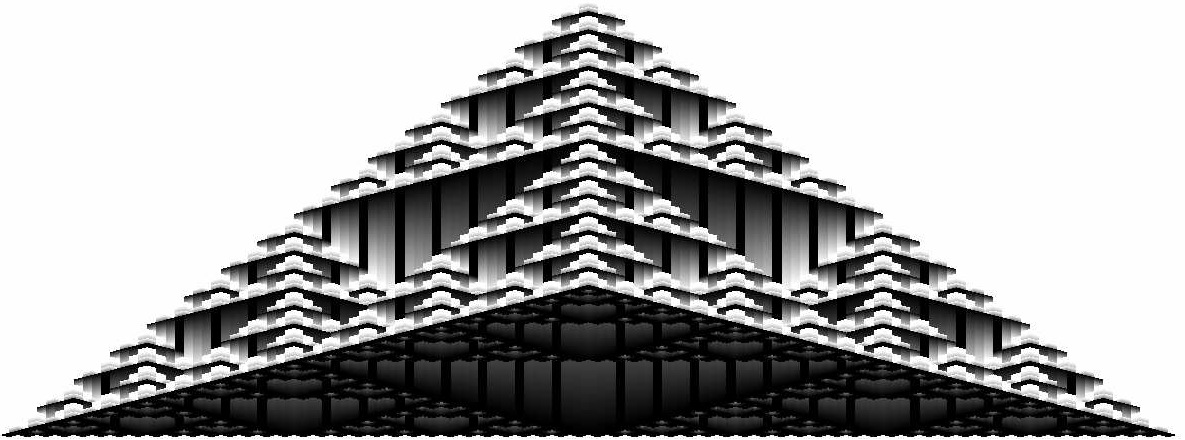
\includegraphics[width=0.9\textwidth]{mycerinus}
\caption{We hadden ook de demonstratie kunnen doen met een tabel, maar tabellen bevatten meestal slechts woorden en volgens figuur \ref{cheops-chephren} zegt een figuur meer dan duizend woorden. Dus hoewel dit bijschrift lang lijkt (nodig om dat inspringen te illustreren), is de figuur nog veel langer.\label{mycerinus}}
\end{center}
\end{figure}

\subsection{Verwijzingen naar tabellen en figuren}

Het is handig wanneer we kunnen verwijzen naar onze tabellen en figuren. Dit gebeurt met het mechanisme uitgelegd in sectie \ref{label-ref} op bladzijde \pageref{label-ref}. We plaatsen een \lcommand{\\label\{labeltjefig\}} in de \lcommand{caption}. Let erop dat dit wel degelijk in de \lcommand{caption} is en niet erbuiten. Dit is logisch: de \lcommand{caption} zorgt voor nummering van de figuur; geen \lcommand{caption}, geen nummering, geen mogelijkheid om de tabel aan te wijzen. Met \lcommand{\\ref\{labeltjefig\}} of \lcommand{\\pageref\{labeltjefig\}} kunnen we refereren naar de \engels{float}.
\npar
In wetenschappelijke teksten is het gebruikelijk dat tabellen en figuren nooit verschijnen voordat ze in de tekst vermeld worden. \latex durft dit nogal eens wel te doen. Wanneer je op het einde van een bladzijde een figuur invoegt, en je hebt er juist voor het invoeren naar verwezen, kan het zijn dat die figuur bovenaan de bladzijde geplaatst wordt, dus voordat ernaar verwezen wordt. \latex gaat dus tekst die in het bronbestand v\'o\'or de figuur staat, in het finale pdf-document n� de figuur plaatsen. Om dit te vermijden, moet de volgende lijn in de \engels{preamble} opgenomen worden:
\begin{llt}
\usepackage{flafter}        % Opdat floats niet zouden voorsteken
\end{llt}
Let er dan wel op dat je eerst naar een figuur of tabel verwijst, vooraleer ze in te brengen in de tekst.

\subsection{Enkele voorbeelden}\label{voorbeeldfloat}

Het is mooi wanneer onze tabellen en figuren gecentreerd staan. Daarom dat we de \engels{floats} in een \lcommand{center} omgeving zetten. Dat centreren moet gebeuren binnen de \engels{float} omgeving (zie voorbeeld hieronder).
\npar
De code nodig om figuur \ref{mycerinus} te genereren is:
\begin{llt}
\begin{figure}[ht]
  \begin{center}
    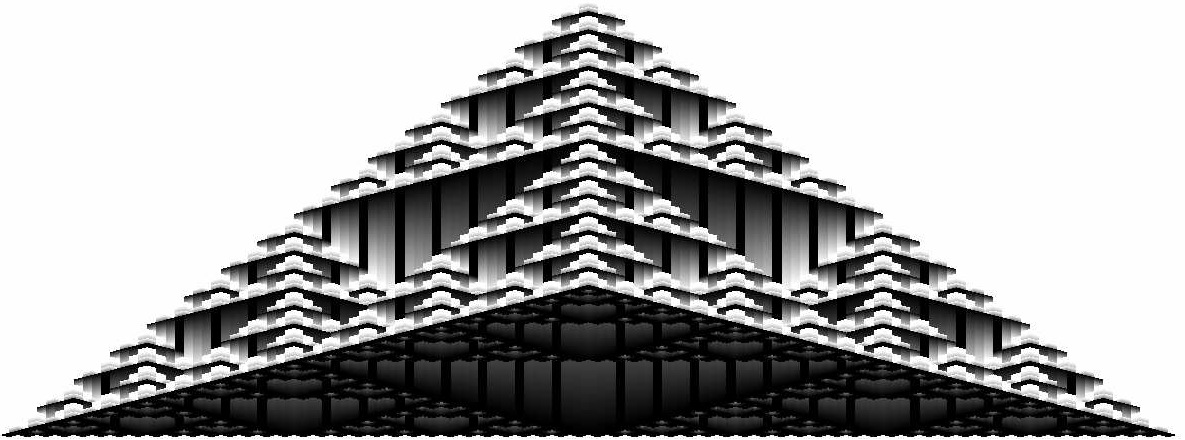
\includegraphics[width=0.9\textwidth]{mycerinus}
    \caption{We hadden ook de demonstratie kunnen doen met een tabel, maar tabellen bevatten meestal slechts woorden en volgens figuur \ref{cheops-chephren} zegt een figuur meer dan duizend woorden. Dus hoewel dit bijschrift lang lijkt (nodig om dat inspringen te illustreren), is de figuur nog veel langer.\label{mycerinus}}
  \end{center}
\end{figure}
\end{llt}
Voor tabellen gebruiken we de \lcommand{table} omgeving. In plaats van een \lcommand{\\includegraphics}, komt er nu een \lcommand{tabular} omgeving. Eventueel kunnen we de \lcommand{tabular} in een apart bestand plaatsen en in onze \lcommand{table} omgeving invoegen met een \lcommand{\\input\{tabelbestandsnaam\}} commando. Vergeet ook niet om de caption v\'o\'or de eigenlijke tabel te defini�ren. Om tabel \ref{letterstijlen} op bladzijde \pageref{letterstijlen} te genereren werd de volgende code gebruikt:
\begin{llt}
\begin{table}[h]
    \begin{center}
    \caption{Hoe verschillende letterstijlen selecteren: met een nieuwe omgeving of met een commando.\label{letterstijlen}}
        \begin{tabular}{l@{\;}l@{\quad}l@{\;}l}
        ... % de verschillende rijen
        \end{tabular}
    \end{center}
\end{table}
\end{llt}

\begin{MinderBelangrijk}
Het bijschrift even breed krijgen als de \engels{float} kan gebeuren met een \lcommand{\\parbox} (de uitleg over parboxen is te vinden op bladzijde \pageref{parbox}):
\begin{llt}
\begin{figure}[ht]
  \begin{center}
    
\includegraphics[width=0.3\textwidth]{tux}
    % De volgende witte lijn is belangrijk: anders komt caption naast figuur!

    \parbox{0.3\textwidth}{\caption{Giza is dood. Leve de Penguin!\label{tux}}}
  \end{center}
\end{figure}
\end{llt}
Het resultaat is te bewonderen in figuur \ref{tux}.
\begin{figure}[ht]
  \begin{center}
    
\includegraphics[width=0.3\textwidth]{tux}
    % De volgende witte lijn is belangrijk: anders komt caption naast figuur!

    \parbox{0.3\textwidth}{\caption{Giza is dood. Leve de Penguin!\label{tux}}}
  \end{center}
\end{figure}
\end{MinderBelangrijk}

\subsection{Nieuw commando om gemakkelijk \engels{floats} in te voegen}

Altijd dat \lcommand{\\begin\{center\}}, \lcommand{\\caption}, \lcommand{\\label} intypen is nogal vermoeiend. Algauw ga je de instellingen van de vorige figuur kopi�ren en wijzig je de figuurnaam, het label en het bijschrift. Lastig, je kan gemakkelijk fouten maken. Veel handiger is als je een commando maakt dat dat allemaal voor jou doet. Wat we eigenlijk wensen, is iets als:
\begin{llt}
\mijnfiguur[plaatsingsopties]{opties-includegraphics}{bestand}{Bijschrift}
\end{llt}
Inderdaad, het is niet echt nodig om een label mee te geven. Als we ervan uitgaan dat elke bestandsnaam geen \engels{slashes} bevat (zie bladzijde \pageref{graphicspath} over het ingeven van de directories waar \latex moet zoeken naar figuren) en uniek is, kunnen we de bestandsnaam gebruiken als label. De plaatsingsopties bepalen waar de figuur moet terechtkomen (zie bladzijde \pageref{plaatsingfloat}); dit is een optioneel argument, daar we een standaardwaarde kunnen gebruiken voor het hele document. De opties voor \lcommand{includegraphics} zijn verplicht. Meestal moet de figuur toch herschaald worden en is een \lcommand{width=xxx} nodig. Dit kan moeilijk dezelfde zijn voor elke figuur.
\npar
Het commando \lcommand{\\mijnfiguur} wordt als volgt gedefinieerd (voor uitleg over het aanmaken van nieuwe commando's verwijzen we naar sectie \ref{commandos} op bladzijde \pageref{commandos}):
\begin{llt}
\newcommand{\mijnfiguur}[4][ht]{
    \begin{figure}[#1]
        \begin{center}
            \includegraphics[#2]{#3}
            \caption{#4\label{#3}}
        \end{center}
    \end{figure}
    }
\end{llt}
Het eerste argument bevat de opties die vertellen waar onze figuur moet geplaatst worden. Standaard proberen we figuren te plaatsen waar ze gedefinieerd worden. Als dat niet lukt, hebben we ze liefst bovenaan een bladzijde. Het tweede argument bevat de opties voor \lcommand{includegraphics}. Het derde argument bevat de bestandsnaam, wat ook het label wordt, en het vierde argument bevat de tekst van het bijschrift.
\npar
Figuur \ref{mycerinus}, zou dus als volgt kunnen geplaatst worden in ons document:
\begin{llt}
\mijnfiguur{width=0.9\textwidth}{mycerinus}{We hadden ook de demonstratie...}
\end{llt}
Wat veel eleganter is dan heel die rompslomp in sectie \ref{voorbeeldfloat}.
\npar
Iets analoogs kan gedaan worden voor tabellen. Er moeten nu geen opties meer meegegeven worden met \lcommand{includegraphics} zodat we slechts drie argumenten hebben (merk ook op dat de caption v\'o\'or de tabelinput komt):
\begin{llt}
\newcommand{\mijntabel}[3][ht]{
    \begin{table}[#1]
        \begin{center}
            \caption{#3\label{#2}}
            \input{#2}
        \end{center}
    \end{table}
    }
\end{llt}
Ingeven van een tabel gebeurt dan als volgt:
\begin{llt}
\mijntabel[hb]{bestand-met-tabel}{Bijschrift bij de tabel.}
\end{llt}

